% TO-DO:  Kolmogorov complexity

\documentclass[17pt]{beamer}
\usepackage[CJKspace]{xeCJK}
%\usepackage{newtxtext,newtxmath}	% use Times Roman font
%\usefonttheme{serif}
\usefonttheme{professionalfonts}
%\setbeamertemplate{theorems}[numbered]
\setbeamertemplate{caption}{\insertcaption} 	% no `Figure' prefix before caption

\mode<presentation> {

%\usetheme{default}
%\usetheme{AnnArbor}
%\usetheme{Antibes}
%\usetheme{Bergen}
%\usetheme{Berkeley}
%\usetheme{Berlin}
%\usetheme{Boadilla}
%\usetheme{CambridgeUS}
%\usetheme{Copenhagen}
%\usetheme{Darmstadt}
%\usetheme{Dresden}
%\usetheme{Frankfurt}
%\usetheme{Goettingen}
%\usetheme{Hannover}
%\usetheme{Ilmenau}
%\usetheme{JuanLesPins}
%\usetheme{Luebeck}
\usetheme{Madrid}
%\usetheme{Malmoe}
%\usetheme{Marburg}
%\usetheme{Montpellier}
%\usetheme{PaloAlto}
%\usetheme{Pittsburgh}
%\usetheme{Rochester}
%\usetheme{Singapore}
%\usetheme{Szeged}
%\usetheme{Warsaw}

%\usecolortheme{albatross}
%\usecolortheme{beaver}
%\usecolortheme{beetle}
%\usecolortheme{crane}
%\usecolortheme{dolphin}
%\usecolortheme{dove}
%\usecolortheme{fly}
%\usecolortheme{lily}
%\usecolortheme{orchid}
%\usecolortheme{rose}
%\usecolortheme{seagull}
%\usecolortheme{seahorse}
%\usecolortheme{whale}
%\usecolortheme{wolverine}

%\setbeamertemplate{footline} % To remove the footer line in all slides uncomment this line
%\setbeamertemplate{footline}[page number] % To replace the footer line in all slides with a simple slide count uncomment this line
\setbeamertemplate{navigation symbols}{} % To remove the navigation symbols from the bottom of all slides uncomment this line
}

\usepackage{graphicx} % Allows including images
\usepackage{verbatim} % comments
% \usepackage{tikz-cd}  % commutative diagrams
% \newcommand{\tikzmark}[1]{\tikz[overlay,remember picture] \node (#1) {};}
% \usepackage{booktabs} % Allows the use of \toprule, \midrule and \bottomrule in tables
% \usepackage{amssymb}  % \leftrightharpoons
\usepackage{wasysym} % frownie face

\newcommand{\vect}[1]{\boldsymbol{#1}}
\newcommand*\sigmoid{\vcenter{\hbox{\includegraphics{sigmoid.png}}}}

\makeatletter
\renewcommand{\boxed}[1]{\fbox{\m@th$\displaystyle\scalebox{0.9}{#1}$} \,}
\makeatother

%---------------------------- make slide margin narrower --------------------------------
\newcommand\Wider[2][3em]{%
	\makebox[\linewidth][c]{%
		\begin{minipage}{\dimexpr\textwidth+#1\relax}
			\raggedright#2
		\end{minipage}%
}%
}

%----------------------------------------------------------------------------------------
%	TITLE PAGE
%----------------------------------------------------------------------------------------

\title[AGI theory]{My AGI theory explained} % The short title appears at the bottom of every slide, the full title is only on the title page

\author{YKY 甄景贤} % Your name
\institute[] % Your institution as it will appear on the bottom of every slide, may be shorthand to save space
{
Independent researcher, Hong Kong \\ % Your institution for the title page
\medskip
\textit{generic.intelligence@gmail.com} % Your email address
}
\date{\today} % Date, can be changed to a custom date

\begin{document}

\frame{\titlepage}

\begin{frame}
\frametitle{Talk summary}
\tableofcontents
\end{frame}

%---------------- this is for when you're using \part's ----------------------------------
%\begin{frame}
%\frametitle{Summary}
%
%{\usebeamerfont*{frametitle} Part I %\usebeamercolor[fg]{frametitle}
% ~ ~ ~ Deep reinforcement learning}
%%\tableofcontents[part=1]
%
%\vspace{1.5cm}
%{\usebeamerfont*{frametitle} Part II %\usebeamercolor[fg]{frametitle}
% ~ ~ ~ Logical structure}
%%\tableofcontents[part=2]
%\end{frame}

%----------------------------------------------------------------------------------------
%	PRESENTATION SLIDES
%----------------------------------------------------------------------------------------

%------------------------------------------------

%\part{title}

\section[Section]{What is inductive bias? ``No free lunch'' theorem}
\frame{\sectionpage}

\begin{frame}
\frametitle{The goal of machine learning}
\begin{itemize}
	\item The goal of machine learning is to search in a \textbf{space} of learning machines, those machines that satisfy certain criteria
	\item For example, among the neural networks of a certain size and shape, find the weights that satisfy an \textbf{objective function}
\end{itemize}
\end{frame}

\begin{frame}
\frametitle{AI Winter}
\begin{itemize}
	\item Generally speaking, bottleneck problem of AI = {\color{red}\textbf{search space too large}}, thus learning too slow
	\item Historically, ``AI Winter'' occurred because \textbf{logic-based} AI learning suffers from combinatorial explosion, and we lacked workable \textbf{heuristics} to tackle it
\end{itemize}
\end{frame}

\begin{frame}
\frametitle{Inductive bias}
\begin{itemize}
	\item Every learning algorithm has its \textbf{inductive bias}
	\item In other words, some regions of the search space would not be searched
	\item Thus bias makes learning faster
	\item But if bias is too strong, the space containing the solution would be cut off \\
	``Throw the baby out with the water''
\end{itemize}
\end{frame}

\begin{frame}
\frametitle{``No free lunch'' theorem}
\fontsize{16}{15}\selectfont
\begin{itemize}
	\item When search space has no \textit{a priori} structure, any inductive bias must be {\color{red}\textbf{good at some problems while bad at others}};  the meaning of ``no free lunch''
	\item For example, vision has the invariance of 3D Euclidean geometry, thus the human visual cortex may have inductive bias for this invariance
	\item Or, human cognition has ``logical'' structure, using this inductive bias may accelerate machine learning of human intelligence
\end{itemize}
\end{frame}

\begin{frame}
\frametitle{Kolmogorov complexity}
\fontsize{16}{15}\selectfont
\begin{itemize}
	\item is {\color{red}\textbf{incomputable}}, but {\color{red}\textbf{approximable}}
	\item The {\color{red}\textbf{semantic distance metric}} between logic propositions is related to it, where one logic deduction step corresponds to 1 unit of semantic distance
	\item Find a set of logic rules, that \textbf{explains} the world, and not deduce false facts, and \# of rules cannot be too large --- these requirements \textit{implicitly} approximate Kolmogorov complexity
\end{itemize}
\end{frame}

\section[Section]{What gives neural networks their power?}
\frame{\sectionpage}

\begin{frame}
\frametitle{Structure of a neural network}
\begin{itemize}
	\item 1 neuron is a \textbf{dot product} followed by a \textbf{non-linearity}:
	\begin{equation}
	\sigmoid \langle \vect{x}, \vect{w} \rangle
	\end{equation}	
	\item The non-linearity can take various forms, \textit{eg}:
	\begin{equation}
	\sigmoid (\xi) = \frac{1}{1 + e^{- \xi}}
	\end{equation}
\end{itemize}
\end{frame}

\begin{frame}
\frametitle{Structure of a neural network}
\begin{itemize}
	\item 1 \textbf{layer} of neurons is a matrix multiplication:
	\begin{equation}
	\sigmoid( \; W \cdot \vect{x} \; )
	\end{equation}	
	\item A neuron network is the function composition $(f \circ f)$ of many {\color{red}layers}:
	\begin{equation}
	[ \sigmoid W ]^L \; \vect{x}
	\end{equation}	
\end{itemize}
\end{frame}

\begin{frame}
\frametitle{Properties of neural networks}
\begin{itemize}
	\item A neural network is a function with many {\color{red}\textbf{parameters}}
	\item It is a \textbf{universal function approximator} [Cybenko 1989]
	\item Its proof can be traced to Weierstrauss's approximation theorem (1885): any continuous function can be uniformly approximated by polynomials
	\item But the proof is {\color{red}independent of depth}
\end{itemize}
\end{frame}

\begin{frame}
\frametitle{Power of NNs comes from depth}
\begin{itemize}
	\item Suppose $\sigmoid W \vect{x}$ is a \textit{cubic} polynomial
	\item Adding each layer is equivalent to:
	\begin{equation}
	 (\mbox{polynomial} \circ \mbox{polynomial})
	\end{equation}
	\item Thus, the resulting polynomial has total degree = $3^L$
	\item In other words, total degree grows  {\color{red}\textbf{exponentially}}
\end{itemize}
\end{frame}

\begin{frame}
\frametitle{Power of NNs comes from depth}
\begin{itemize}
	\item \textbf{代数基本定理}:多项式 \textbf{次数} = 曲线 跨过 $x=0$ 多少次
	\begin{equation}
	\vcenter{\hbox{\includegraphics[scale=0.4]{../2018/zero-crossings.png}}}
	\end{equation}
	\item 高维: 曲面 对 分类空间 {\color{red}分割成 多少块}
\end{itemize}
\end{frame}

\begin{frame}
\frametitle{Power of NNs comes from depth}
\begin{itemize}
	\item 这和 VC-dimension 道理一样 [Vapnik–Chervonenkis 1971] 
	\item VC-dimension = 函数 能将 空间 分割成多少块
	\item 多层 神经网络 的 VC-dim 是 $O(N \log N)$ 其中 $N$ 是 网络参数 的总个数,但证明用的是不连续的 阀函数
	\item 我估计 VC-dim 会是 指数增长的,但未有证明
\end{itemize}
\end{frame}

\begin{frame}
\frametitle{Power of NNs comes from depth}
\begin{itemize}
	\item VC-dim {\color{red}\textbf{指数增长}} 的意义,表示 神经网络 能 代表 一些 非常复杂的 \textbf{函数家族}
	\item 而 神经网络 的参数个数 相对地 很少,可以在 电脑上实现
\end{itemize}
\end{frame}

\begin{frame}
\frametitle{Revelation from convolution networks}
\begin{itemize}
	\item Yann LeCun 在 1989 发明了 ConvNet,触发了 机器视觉 的革命,最近得了 Turing 奖
	\begin{equation}
	\nonumber
	\vcenter{\hbox{\includegraphics[scale=0.25]{Yann-LeCun.jpg}}}
	\end{equation}
\end{itemize}
\end{frame}

\begin{frame}
\frametitle{Revelation from convolution networks}
\begin{itemize}
	\item CNN 将普通 NN 的 点积 用 卷积 代替:
	\begin{equation}
	\boxed{\mbox{点积}} \quad \sigmoid \langle \vect{x}, \vect{w} \rangle \rightsquigarrow \sigmoid( f * g ) \quad \boxed{\mbox{卷积}}
	\end{equation}
	\item 而 卷积 具有 {\color{red}\textbf{平移 不变性}},有利於 视觉:
	\begin{equation}
	T_x(f) * g = T_x( f * g )
	\end{equation}
	\item 这是一种 \textbf{归纳偏好},令 学习 更快
\end{itemize}
\end{frame}

\begin{frame}
\frametitle{Revelation from convolution networks}
\begin{itemize}
	\item 其实 \textbf{视觉} 需要的是 \textbf{仿射} (affine) 不变性,它包括 平移、旋转、放大缩小 等
	\item 但 似乎 单单是 平移不变性 所带来的 \textbf{学习加速},已足以令 CNN 在 2012 年超越了人类水平
	\item 可见,\textbf{归纳偏好} 在 深度学习 里 仍然是很有用的
\end{itemize}
\end{frame}

\section{Turing machines and universal logic}
\frame{\sectionpage}

\begin{frame}
\frametitle{Finite state machines}
\begin{itemize}
	\item 有限自动机 通常用一些 tuple 定义(从略),例如:
	\begin{equation}
	\vcenter{\hbox{\includegraphics[scale=0.7]{finite-state-machine.png}}}
	\end{equation}
	\item 这个 自动机 {\color{red}\textbf{接受}} ``a'', ``aba'', ``ababa...'' 等 字串
\end{itemize}
\end{frame}

\begin{frame}
\frametitle{Finite state machines}
\Wider[1em]{
\begin{itemize}
	\item 有限自动机 可以接受 $\mbox{a}^m \mbox{b}^n$ 这种字串,$m$ 和 $n$ 不同
	\item 但它不能接受 $\mbox{a}^k \mbox{b}^k$ 这种字串,因为它里面没有办法「记住」$k$ 是多少次
	\item 有限自动机 能辨认的 \textbf{语言},称作 \textbf{regular languages}
	\item Noam Chomsky 在 1950s 定义,他是计算机科学家 + 语言学家,现在主要谈政治,从左派角度批评美国资本主义
\end{itemize}
}
\end{frame}

\begin{frame}
\frametitle{Turing machines}
	Turing 机 = 有限自动机 + 无限长 的 {\color{red}\textbf{记忆磁带}} (每个 state 可以 读/写 一个字符)\\
	\begin{equation}
	\label{fig:Turing-machine}
	\includegraphics[scale=0.6]{../AGI-16/Turing-machine.png}
	\end{equation}
\end{frame}

\begin{frame}
\frametitle{Turing machines}
\begin{itemize}
	\item 亦即是说: 有限自动机 + 无限读写带 = 可以计算任何函数,此即 Church-Turing 假设
	\item Turing 机 等价於 $\lambda$-calculus、combinatory logic、cellular automata、game of life、recurrent 神经网络、等
\end{itemize}
\end{frame}

\begin{frame}
\frametitle{Alan Turing (1912-1954)}
\begin{itemize}
	\item Turing 是一个 远超越於时代 的人
	\item 他考虑过 神经网络 作为学习机器
	\item 也考虑过 进化算法 (evolutionary algorithms)
	\item 而当时 1940s 还未有电脑 --- 电脑是他发明的!
	\item {\color{red}他求出所有\textbf{可计算函数}的形式,从而将AI的问题 \textbf{限制} 在一框框内} 
\end{itemize}
\end{frame}

\begin{frame}
\frametitle{Recurrent neural networks}
	其实一个 RNN 可以看成类似 (\ref{fig:Turing-machine}) 的结构:
	\begin{equation}
	\includegraphics[scale=0.6]{RNN-as-Turing-machine.png}
	\end{equation}
	重点是 hidden state 可以储存计算的 {\color{red}中途结果},令 RNN 也变成 Turing 机
\end{frame}

\section[Section]{Structure of classical AI systems}
\frame{\sectionpage}

\begin{frame}
\frametitle{John McCarthy (1927-2011)}
\begin{itemize}
	\item 「AI 之父」
	\item 1956年 在 Dartmouth 第一次举行「人工智能」会议
	\item 开创了 使用 {\color{red}\textbf{数理逻辑}} 作为 AI 的 \textbf{知识表述} (knowledge representation)
	\item 晚年研究 \textbf{改写系统} (term rewriting systems),是一种更 \textbf{广义} 的逻辑
\end{itemize}
\end{frame}

\begin{frame}
\frametitle{The world of logical structures}
\Wider[2em]{
\includegraphics[scale=0.43]{../2018/world-of-logical-structures.png}}
\end{frame}

\begin{frame}
\frametitle{Propositional vs predicate logic}
\begin{itemize}
	\item 最重要是 搞清 \textbf{命题逻辑} 和 一阶 \textbf{谓词逻辑} 的区别
	\item 命题逻辑:$P_1 =$ 「昨天下雨」 \\ \hspace{3cm} $P_2 =$「今天下雨」\\
		{\color{red}命题 没有 \textbf{内部结构}}
	\item 谓词逻辑:$P_3 =$ 下雨(北京,前天)
	\item 谓词 有 \textbf{代入}(substitution) 的复杂性
\end{itemize}
\end{frame}

\begin{frame}
\frametitle{Architecture of logic-based AI systems}
这个 架构 很重要,就像 蒸汽机 时代 的 Carnot cycle(卡诺循环):
\begin{equation}
\label{fig:LBAI-architecture}
\vcenter{\hbox{\includegraphics[scale=0.5]{LBAI-architecture.png}}}
\end{equation}
\end{frame}

\begin{frame}
\frametitle{What is a logic rule?}
\begin{itemize}
	\item 举例: 爱一个人 但他不爱你 则失恋
	\begin{equation}
	\heartsuit(x,y) \wedge \neg \heartsuit(y,x) \Rightarrow \frownie{}(x)
	\end{equation}
	\item 这是一条 rule,变量 $x,y$ 需要 {\color{red}\textbf{代入}} 适当的个体,例如 $\{x \setminus \mbox{John}, y \setminus \mbox{Mary} \}$
	\item 寻找 代入 的算法叫 \textbf{matching}  或 \textbf{unify}
\end{itemize}
\end{frame}

\begin{frame}
\frametitle{SOAR cognitive architecture}
\Wider[1em]{
\begin{itemize}
	\item SOAR 是一个著名的 \textbf{认知架构}
	\item 基本上 它根据 working memory 寻找 可以\textbf{发动}的 rules,类似图(\ref{fig:LBAI-architecture})
	\item 它用 \textbf{Rete} 算法 快速地搜寻 可用的 rules,这是经典 AI 里的重要算法(\textit{rete} 在拉丁文的意思是「网状」)
	\item 鉴於中国AI的后起之秀,视野不够广阔,故补充一些基础知识
\end{itemize}
}
\end{frame}

\begin{frame}
\frametitle{My theory}
\Wider[2em]{
\begin{itemize}
	\item 我的理论里,rules 和 matching 机制,都 \textbf{纳入} 到 神经网路 里
	\item 神经网络 这件武器,优点是 可以 逼近 很复杂的 mappings,它是现时最强的 机器学习 方法
	\item 我将 逻辑结构 松弛 (relax),务求做到足够的 归纳偏好 即可
	\item 这理论中最关键的元件,是 symmetric 神经网络
\end{itemize}
}
\end{frame}

\begin{frame}
\frametitle{Commutativity of logic conjunctions}
\Wider[1em]{
\begin{itemize}
	\item $\wedge$ 的交换律 可能是 逻辑 中最重要的规律:
	\begin{equation}
	\mbox{肚饿} \wedge \mbox{没钱} \Leftrightarrow \mbox{没钱} \wedge \mbox{肚饿}
	\end{equation}
	\item 也可以理解为: 从 前提 推导出 结论,前提中 命题的 {\color{red}\textbf{次序}} 应该没有关系,甚至可以夹杂无关的命题
	\item 交换律 抽象了 逻辑命题 的结构,类似 抽象代数 中,交换群(又叫 阿贝尔群,纪念 Abel)的重要性
\end{itemize}
}
\end{frame}

\begin{frame}
\frametitle{Symmetric neural networks}
\begin{itemize}
	\item 卷积 神经网络 具有 平移不变性
	\item 类似地,{\color{red}\textbf{对称}}神经网络 具有 交换不变性 (permutation invariance)
	\item 它可以透过 weight-sharing 来实现,类似 卷积层 的权重共享
	\item SymNet :逻辑 $\approx$ ConvNet :视觉
\end{itemize}
\end{frame}

\section*{结论:中国会不会有自主研发的 AGI?}

\begin{frame}
\frametitle{Will China build its own AGI?}
\Wider[1em]{
\begin{itemize}
	\item 日本 在1980年代 研发 第5代电脑 的失败,可以作为借鉴
	\item 地球的资源有限,科技发展 往往是国与国之间 竞争的结果
	\item 在美国有歧视中国的人,中国内部也有拖后腿、倒向外国的人,但在美国也有帮过我的朋友
	\item 所以我比较支持 建立全球化的 AGI 项目
\end{itemize}
}
	\begin{center}
		多谢收看 \smiley{}
	\end{center}
\end{frame}

\begin{comment}

\begin{frame}
\frametitle{References}
\footnotesize{
\begin{thebibliography}{99} % Beamer does not support BibTeX so references must be inserted manually as below
\bibitem[]{} Bart Jacobs (1999)
\newblock Categorical logic and type theory
% \newblock \emph{North Holland, Studies in logic} v141.

\bibitem[]{} Robert Goldblatt (2006)
\newblock Topoi -- the categorical analysis of logic

\end{thebibliography}
}
\end{frame}

\begin{frame}
We're looking for developers to implement a prototype.

\vspace*{1cm}
\Large{\centerline{Thank you}}

%\vspace*{1cm}
%\Large{\centerline{The End}}
\end{frame}

\end{comment}

\end{document} 